% Chapter 4

\chapter{Methodology} % Main chapter title

\label{Chapter4} % For referencing the chapter elsewhere, use \ref{Chapter1} 

\lhead{Chapter 4. \emph{Drawings}} % This is for the header on each page - perhaps a shortened title

%----------------------------------------------------------------------------------------
\section{Overview}
The Dynamic Energy Map is created for a conceptual urban environment
with the following properties:
\begin{enumerate}[i.]
\item Of realistic building density and land use pattern.
  
  To achieve this, the current study used a redevelopment project at
  Lower Hill District, Pittsburgh, PA~\cite{Ramesh2013} as a
  prototype.  The land use of the conceptual urban environment is
  created based on extracted topological patterns from this
  redevelopment projec.

\item The number of buildings in the model represents a typical
  community that can be served by a district energy
  system~\cite{IDEA2012}.
  
  To achieve this, the original model created under crateria i. is
  duplicated and thus there are in total 68 buildings within the
  community. This rangge is within the range of a typical district
  energy system service capacity of 50 to 150~\cite{IDEA2012}.

\end{enumerate}

The inputs to the dynamic energy map include the hourly energy
consumption data and the urban environment layout. For the conceptual
setting, the energy data is retrieved from the simulation of DOE
Benchmark buildings of new construction which comply with ASHRAE
90.1-2004 Standard~\cite{DOE2015}.

The output of the dynamic energy map is a sequence of 2D or 3D energy
choropleth map images.

An interface is designed to provide an interactive inspection of the
map image sequence and the corresponding energy data plot of a single
buildings, building groups and the community that assists:
\begin{enumerate}[i.]
\item Comparing heating and cooling demand to identify energy recovery
  opportunities
\item Comparing heating and electricity demand to size co-generation
  system
\end{enumerate}

By replacing the simulated hourly energy demand data with actual
metered energy consumption data and the conceptual layout with a real
urban environment layout, the same method can be directly applied to
the analysis of a real project.

\begin{figure}[h!]
  \centering
  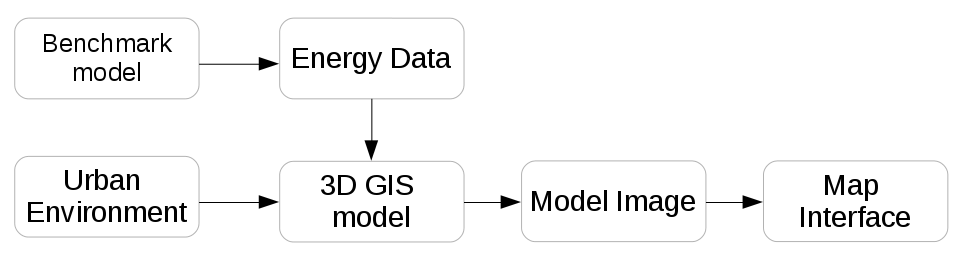
\includegraphics[width=0.7\linewidth]{flow.png}
  \caption[General Work Flow]{General Work Flow}
  \label{fig:flow}
\end{figure}

Details in input output data and the interface design process will be
explained in more details in the following sections.
\newpage
\section{Input}
\subsection{Benchmark Models and Energy Data}
In the Lower Hill District project, the DOE benchmark buildings were
substituted for buildings in the community model in the district
system feasibility analysis. This approach allows for a fast initial
assessment of the district system~\cite{baird2014}.

Following the same approach, the energy profile used in the current
study is retrieved from simulation results of commercial building
benchmark buildings developed by U.S. Department of Energy
(DOE)~\cite{DOE2015}. There are 16 building types in the benchmark
models (\fref{tab:doeModel}). The building types involved in the
current project include: Large Office (LO), Medium Office (MO), Small
Office (SO), Stand-alone Retail (SR), Supermarket (SU), Quick Service
Restaurant (QR), Full Service Restaurant (FR), Large Hotel (LH) and
Midrise Apartment (MA). The two-letter shorthand in the parenthesis
after each building type is used in the building label for the dynamic
map display. The general information for the benchmark buildings are
shown in \tref{tab:doeModel}:

\begin{table}[h!]
  \centering
  \begin{tabular}{l|l|c|c}
    \hline
Building Type Name&Shorthand&  Floor Area (ft2)    & Number of Floors\\
    \hline
Large Office	         &LO&  498,588	      & 12\\
Medium Office	         &MO&  53,628	      & 3\\
Small Office	         &SO&  5,500	      & 1\\
Warehouse	         &WH&  52,045	      & 1\\
Stand-alone Retail       &SR&  24,962	      & 1\\
Strip Mall	         &SM&  22,500	      & 1\\
Primary School	         &PS&  73,960	      & 1\\
Secondary School         &SS&  210,887	      & 2\\
Supermarket	         &SU&  45,000	      & 1\\
Quick Service Restaurant &QR&  2,500          & 1\\
Full Service Restaurant  &FR&  5,500          & 1\\
Hospital	         &HO&  241,351	      & 5\\
Outpatient Health Care   &OP&  40,946	      & 3\\
Small Hotel	         &SH&  43,200	      & 4\\
Large Hotel	         &LH&  122,120	      & 6\\
Midrise Apartment        &MA&  33,740	      & 4\\
    \hline
\end{tabular}
\caption{DOE Benchmark Building General Information~\cite{DOE2015}}
\label{tab:doeModel}
\end{table}

The benchmark buildings comply with the ASHRAE Standard 90.1-2004. The
HVAC system types are shown in \tref{tab:hvac}. The major heating
systems of the benchmark buildings are furnace and boilers, except
that the small hotel and the warehouse has individual space heaters
other than furnaces. The cooling systems are chillers for Large Hotel
(air-based) and Large Office (water-based) and PACU (packed
air-conditioning unit) for other building types.~

\begin{table}[h!]
\centering
\scriptsize
\caption{Benchmark Building HVAC System}
\label{tab:hvac}
%\begin{tabular}{l|p{3cm}|p{4cm}|p{4cm}}
\begin{longtable}{p{2cm}|p{2cm}|p{4cm}|p{4cm}}
  \hline
  & Heating                                & Cooling                                                                     & Air                                                     \\
  \hline
  \hline
  Small Office             & Furnace                                & PACU (packed air-conditioning unit)                                         & SZ CAV (single-zone constant air volume)                \\
  \hline
  Medium Office            & Furnace                                & PACU (packed air-conditioning unit)                                         & MZ VAV (multizone variable air volume)                  \\
  \hline
  Large Office             & Boiler                                 & Chiller (2) water cooled                                                    & MZ VAV (multizone variable air volume)                  \\
  \hline
  Primary School           & Boiler                                 & PACU (packed air-conditioning unit)                                         & CAV (constant air volume)                               \\
  \hline
  Secondary School         & Boiler                                 & Chiller (2) air cooled                                                      & MZ VAV (multizone variable air volume)                  \\
  \hline
  Stand-Alone Retail       & Furnace                                & PACU (packed air-conditioning unit)                                         & SZ CAV (single-zone constant air volume)                \\
  \hline
  Strip Mall               & Furnace                                & PACU (packed air-conditioning unit)                                         & SZ CAV (single-zone constant air volume)                \\
  \hline
  Suprmarket               & Furnace                                & PACU (packed air-conditioning unit)                                         & SZ CAV (single-zone constant air volume)                \\
  \hline
  Quick Service Restaurant & Furnace                                & PACU (packed air-conditioning unit)                                         & CAV (constant air volume)                               \\
  \hline
  Full Service Restaurant  & Furnace                                & PACU (packed air-conditioning unit)                                         & SZ CAV (single-zone constant air volume)                \\
  \hline
  Small Hotel              & ISH (individual space heater), furnace & IRAC (individual room air conditioner), PACU (packed air-conditioning unit) & SZ CAV (single-zone constant air volume)                \\
  \hline
  Large Hotel              & Boiler                                 & Chiller (2) air cooled                                                      & FCU (Fan Coil Unit) and VAV (variable air volume)       \\
  \hline
  Hospital                 & Boiler                                 & Chiller (2) water cooled                                                    & CAV (constant air volume) and VAV (variable air volume) \\
  \hline
  OutPatient Healthcare    & Furnace                                & PACU (packed air-conditioning unit)                                         & CAV (constant air volume) and VAV (variable air volume) \\
  \hline
  Warehouse                & ISH (individual space heater), furnace & PACU (packed air-conditioning unit)                                         & SZ CAV (single-zone constant air volume)                \\
  \hline
  Midrise Apartment        & Furnace                                & PACU-SS                                                                     & SZ CAV (single-zone constant air volume)               \\
  \hline
\end{longtable}
\end{table}

\pagebreak
\subsubsection{Input for Identifing Energy Recovery
  Opportunities}\label{sec:inputRecover}
The major heat rejection sources include heating mode heat rejection
and cooling mode heat rejection. The heat rejection in heating mode
happens during the process of the mixing of conditioned and outside
air. This source of heat rejection is more difficult to capture and is
thus left out from the energy recovery potential calculation in this
study. The current study will only focus on the cooling induced heat
reject. 

The heat rejection in cooling mode happens during the condensing
process when the high temperature refrigerant gas condenses with one
of the following heat rejection forms~\cite{Bhatia2015}:
\begin{itemize}
\item Air cooled unit: ambient air is blown through condensing coils
  and removes heat from the gas refrigerant.
\item Cooling tower: cooled water flow past the condensing unit and
  takes away the heat from the gas refrigerant. The water is then
  cooled through evaporation.
\item Fluid cooler: water is sprayed on the condensing coil with fan
  forced air flowing in the opposite direction. It causes evaporative
  cooling effect that takes away the heat from the gas refrigerant.
\end{itemize}
The ``condenser total heat of rejection''~\cite{Bhatia2015} (THR) in
the condensing process equals to the ``net refrigeration effect''
~\cite{Bhatia2015}(RE, the hourly cooling demand), plus the compressor
input, it can be represented with the following equation~\cite{Bhatia2015}:

\begin{equation}\label{eq:reject}
THR = RE * f 
\end{equation}

$f$ is the ``Heat Rejection Factor'' and it is typically between 1.15
and 1.25~\cite{Bhatia2015}. The water-based system has heat rejection
factor closer to 1.15 and the air-based system closer to
1.25~\cite{Bhatia2015}.

To help users identify energy recovery opportunities, the energy
information needed to retrieve include: space heating energy demand
and space cooling energy demand. The space cooling demand (RE in
\eref{eq:reject}) is an indicator for heat rejection that could be
recovered and shared within a single building or a building group.

From \tref{tab:heatFuel}, Large Hotel, Medium Office, Midrise
Apartment, OutPatient Healthcare, Small Hotel and Stand-alone Retail
use both electricity and natural gas for space heating, the rest of
the building types uses only natural gas for space heating. We thus
use the EnergyPlus simulation output parameters
``heating:electricity'' and ``heating:gas'' to represent the space
heating demand of reference buildings.
\begin{table}[h]
\centering
\caption{Annual Total Heating Demand by Fuel Type~\cite{DOE2015}}
\label{tab:heatFuel}
\begin{tabular}{lll}
  \hline
                       & Electricity {[}kBtu{]} & Gas {[}kBtu{]} \\
  \hline
  \hline
FullServiceRestaurant  & 0.0                    & 856637.1       \\
Hospital               & 0.0                    & 14045664.0     \\
LargeHotel             & 843.6                  & 2960506.8      \\
LargeOffice            & 0.0                    & 4741180.3      \\
MediumOffice           & 450791.3               & 192226.8       \\
MidriseApartment       & 56.9                   & 494959.6       \\
OutPatient             & 199581.9               & 2881638.9      \\
PrimarySchool          & 0.0                    & 1579186.5      \\
QuickServiceRestaurant & 0.0                    & 383297.2       \\
SecondarySchool        & 0.0                    & 7746443.0      \\
SmallHotel             & 52129.9                & 450393.2       \\
SmallOffice            & 0.0                    & 66631.5        \\
Stand-aloneRetail      & 6966.5                 & 976583.4       \\
StripMall              & 0.0                    & 1013188.1      \\
SuperMarket            & 0.0                    & 3043905.2      \\
Warehouse              & 0.0                    & 1039850.2     \\
  \hline
\end{tabular}
\end{table}

\begin{figure}[h!]
  \centering
  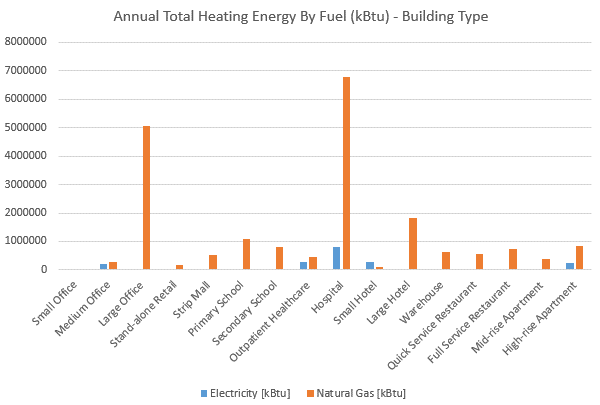
\includegraphics[width=0.7\linewidth]{heatFuel.png}
  \caption[Heating Fuel]{Heating Fuel}
  \label{fig:heatFuel}
\end{figure}
Electricity is the only fuel used for space cooling~\cite{DOE2015},
thus the EnergyPlus output parameter ``cooling:electricity'' is used
to represent space cooling demand. According to the suggested heat
rejection factor~\cite{Bhatia2015}, the heat recovery potential will
be calculated with $f = 1.15$ for Large Office and Hospital, and
$f = 1.25$ for the remaining building types:
\begin{equation}\label{eq:recover}
\text{Heat Recovery Potential} = \text{cooling:electricity} \times f
\end{equation}

In summary, to facilitate identification of energy recovery
opportunities for single buildings and within building groups, the
hourly ``heating:electricity'', ``heating:gas'' and
``cooling:electricity'' output will be extracted from energyPlus
simulation of DOE Commercial benchmark buildings.

\subsubsection{Input for Sizing District Co-generation
  System}
For the sizing of a district co-generation system, the relevant
information needed are the total heating demand, and the total
electricity demand. The general principle used in Lower Hill District
project ~\cite{baird2014} is to use the minimum total heat demand
(space heating and service hot water) over time to assess the minimum
capacity of electricity generation ($E_{heat}$) such that its heat
bi-product from electricity generation will always be consumed. The
maximum total electricity demand ($E_{elec}$) is used for assessing
the capacity of a backup system or a second phase system development
by $C_{backup} = E_{elec} - E_{heat}$ where $C_{backup}$ is the
capacity of electricity generation for the backup system or
second-phase development.

Heating demand assessed in the sizing of co-generation system is
different from the energy recovery use case in \sref{sec:inputRecover}
. It contains the space heating demand and the service hot water
demand. From the summary files of benchmark models, the fuel used for
providing service hot water is natural gas for all building types
(\tref{tab:hotWater})

The output parameter ``electricity:facility'' was extracted to
represent the total electricity demand.

\begin{table}[h!]
\centering
\caption{Service Hot Water by Fuel Type}
\label{tab:hotWater}
\begin{tabular}{l|l|l}
  \hline
                       &  Electricity {[}kBtu{]} & Gas {[}kBtu{]} \\
  \hline
  \hline
FullServiceRestaurant  & 0 & 253664.3       \\
Hospital               & 0 & 719402.7       \\
LargeHotel             & 0 & 6793934.2      \\
LargeOffice            & 0 & 231381.1       \\
MediumOffice           & 0 & 34178.3        \\
MidriseApartment       & 0 & 289719.3       \\
OutPatient             & 0 & 44054.5        \\
PrimarySchool          & 0 & 174768.0       \\
QuickServiceRestaurant & 0 & 82071.5        \\
SecondarySchool        & 0 & 441512.2       \\
SmallHotel             & 0 & 394017.1       \\
SmallOffice            & 0 & 10928.3        \\
Stand-aloneRetail      & 0 & 0.0            \\
StripMall              & 0 & 0.0            \\
SuperMarket            & 0 & 23799.7        \\
Warehouse              & 0 & 0.0            \\
  \hline
\end{tabular}
\end{table}

\pagebreak
\subsection{Simulation Data Analysis of the benchmark
  models}\label{boxPlot}
The output of EnergyPlus simulation of 16 benchmark buildings are
read, processed and plotted with a python program. The data loading
and processing utility is used in both data analysis and the dynamic
plot in the interface design.

The energy output retrieved from EnergyPlus include ``Heating:Gas'',
``Heating:Electricity'', ``Cooling:Electricity'', ``Water
Heater:WaterSystems:Gas'' and ``Electricity:Facility''. This section
will include some basic aggregated analysis of the data distribution.
The meaning of each output variable is listed in
\tref{tab:outputMeaning}:
\begin{table}[h!]
\centering
\caption{Table of EnergyPlus output and their meaning}
\label{tab:outputMeaning}
\begin{tabular}{l|l}
  \hline
EnergyPlus Output            & Meaning\\
  \hline
  \hline
Heating:Gas                  & Total gas for space heating         \\
Heating:Electricity          & Total electricity for space heating \\
Water Heater:WaterSystem:Gas & Total gas for service hot water     \\
Cooling:Electricity          & Total electricity for space cooling \\
Electricity:Facility         & Total electricity                  \\
  \hline
\end{tabular}
\end{table}

\subsubsection{Single Output}
By analysing the EnergyPlus ~\cite{EnergyPlus2015} simulation result
of the output above, we anticipate to gain a basic understanding of
the energy profile data distribution involved in the current
project. We would also want to use this as a basis to compare with the
additional analysis one can performed in a dynamic energy map in the
following sections.

To analyse general distribution of each output variable, we created a
box plot for each of the five variables. By analyzing each single
output, we discovered a great difference between different building
types. 

Hourly gas heating demand of the benchmark buildings range from 0 to
14000 kBtu. The majority (75\%) of all hourly consumption are below
2000 kBtu. All building types have a large amount of outliers above
the 75\% quartile. This indicates gas heating demand of all building
types are severely right skewed. Hospital has the highest median gas
heating demand of about 1100 kBtu. Outpatient Health Care has the
second larges hourly gas heating demand. In terms of peak demand,
Secondary School and Large Office have the highest peak hourly gas
heating demand (\fref{fig:HG}).
\begin{figure}[h!]
  \centering
  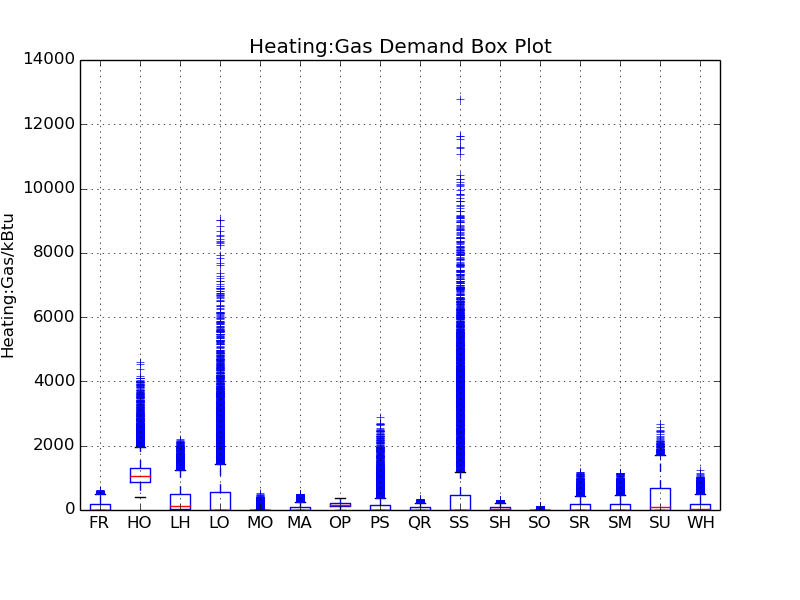
\includegraphics[width=0.7\linewidth]{HG}
  \caption[Heating:Gas Box Plot]{Heating:Gas Box Plot}
  \label{fig:HG}
\end{figure}%

Hourly hot water demand of the benchmark buildings range from 0 to
2500 kBtu, about 1/6 of the range of space heating gas demand. Most
buildings have median hot water hourly demand below 100 kBtu, except
that the median hot water demand of Large Hotel is around 700
kBtu. From \tref{tab:hotWater}, we can see that Stand-alone Retail,
Strip Mall and Warehouse has zero demand for service hot water. Large
Hotel also have a large amount of outliers above the 75\%
quartile. This indicates gas hot water demand of the Large Hotel is
severely right skewed. Hospital has the second largest median gas hot
water demand of about 100 kBtu. Large Hotel also stands out in peak
demand. (\fref{fig:WH}).
\begin{figure}[h!]
  \centering
  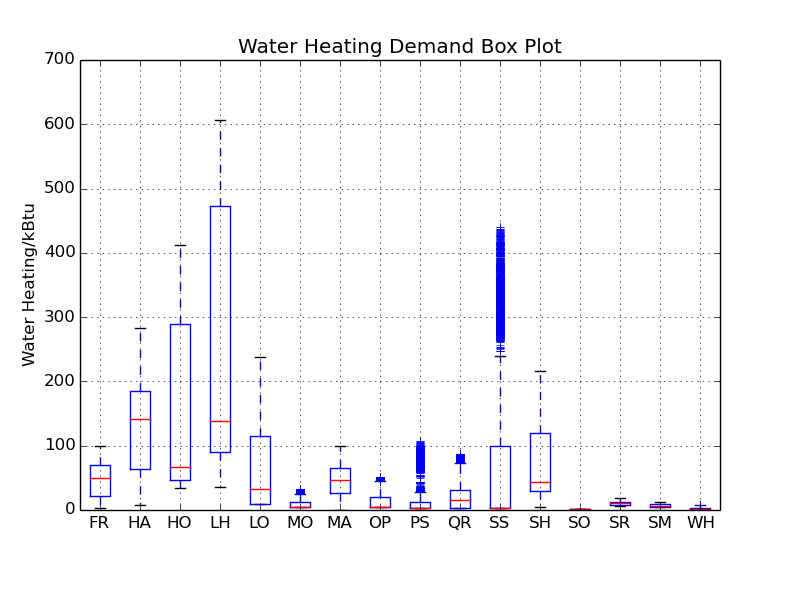
\includegraphics[width=0.7\linewidth]{WH}
  \caption[Water Heater:WaterSystem:Gas Box Plot]{Water
    Heater:WaterSystem:Gas Box Plot}
  \label{fig:WH}
\end{figure}%

From \tref{tab:heatFuel}, only Large Hotel, Medium Office, Midrise
Apartment, OutPatient Healthcare, Small Hotel and Stand-alone Retail
use electricity besides natural gas for space heating. Hourly
electricity heating demand of these buildings range from 0 to 1000
kBtu. All of them has nearly zero median electricity heating demand
and a large amount of outliers above (except for Midrise Apartment)
the 75\% quartile. This indicates electricity heating demand of all
the five building types are severely right skewed. Medium Office has
the highest hourly electricity heating peak demand and Outpatient
Healthcare has the second largest hourly electricity heating peak
demand (\fref{fig:HE}).

\begin{figure}[h!]
  \centering
  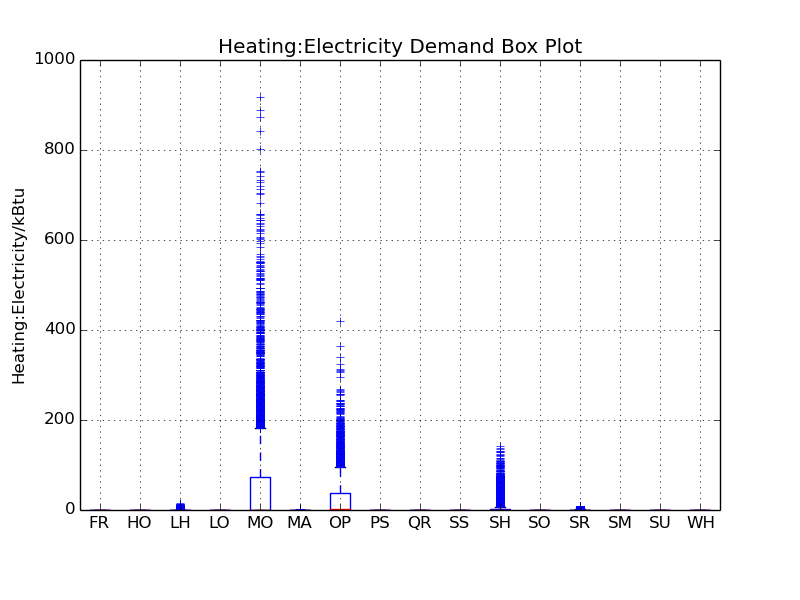
\includegraphics[width=0.7\linewidth]{HE}
  \caption[Heating:Electricity Box Plot]{Heating:Electricity Box Plot}
  \label{fig:HE}
\end{figure}% 

Hourly cooling demand benchmark building types range from 0 to 3000
kBtu, which is about 20\% of that of the peak gas heating demand. The
hospital has the largest median cooling demand of about 1500
kBtu. Large Hotel has the second largest median cooling demand. Both
Hospitals and Large Hotels do not have outliers, indicating their
hourly cooling demand distributions are less skewed. On the contrary,
all other building types have a large amount of outliers above the
75\% quartile, indicating a severe right skew for their hourly cooling
demand distribution. There are four building types with non-zero
median hourly cooling demand: Hospital, Large Hotel, Outpatient Health
Care and Small Hotel. This means they need space cooling for at least
50\% of the year. The constant cooling demand creates the
opportunities for energy recovery of cooling induced reject heat. The
building types with zero median hourly cooling demand then require
cooling only in the cooling season. In terms of hourly cooling peak
demand, the Secondary School has the highest peak demand of about
2700kBtu and Hospital has the second largest peak
demand(\fref{fig:CE}).
\begin{figure}[h!]
  \centering
  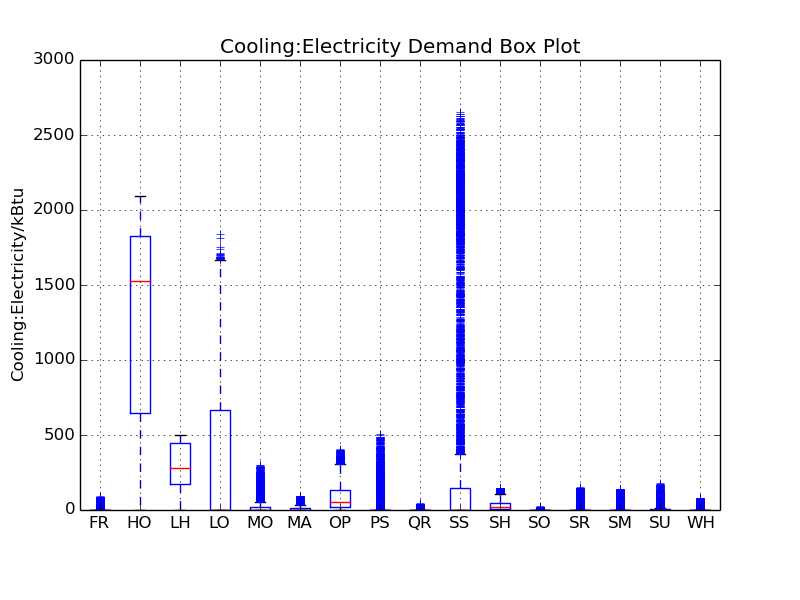
\includegraphics[width=0.7\linewidth]{CE}
  \caption[Cooling:Electricity Box Plot]{Cooling:Electricity Box Plot}
  \label{fig:CE}
\end{figure}%

The hourly electricity demand of benchmark buildings range from 0 to
6000 kBtu, which is about 40\% of that of the peak heating
demand. Comparing with other output variables, the electricity demand
distribution has less outliers in general. The Hospital has the
largest median hourly electricity demand (about 3400 kBtu). The Large
Office has the second largest median hourly electricity demand (about
1800 kBtu). Secondary School has the Largest electricity hourly peak
demand.

\begin{figure}[h!]
  \centering
  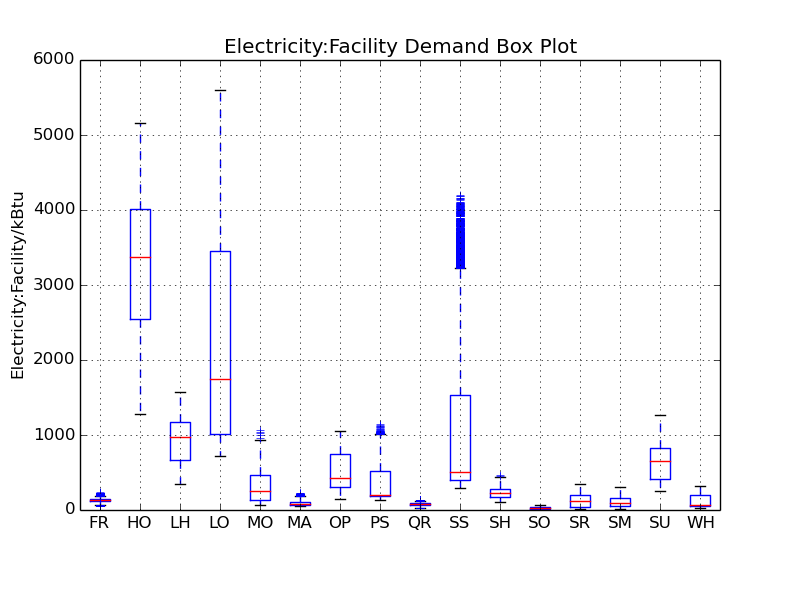
\includegraphics[width=0.7\linewidth]{EF}
  \caption[Electricity:Facility Box Plot]{Electricity:Facility Box
    Plot}
  \label{fig:EF}
\end{figure}%

\subsubsection{Space Heating Demand vs. Space Cooling Demand}
Hourly space heating demand of the benchmark buildings mainly closely
follows the distribution of gas heating demand, with minor demand
increase in Medium Office and Outpatient Health Care (\fref{fig:SH}).

\begin{figure}[h!]
  \centering
  \begin{subfigure}{0.4\textwidth}
  \centering
  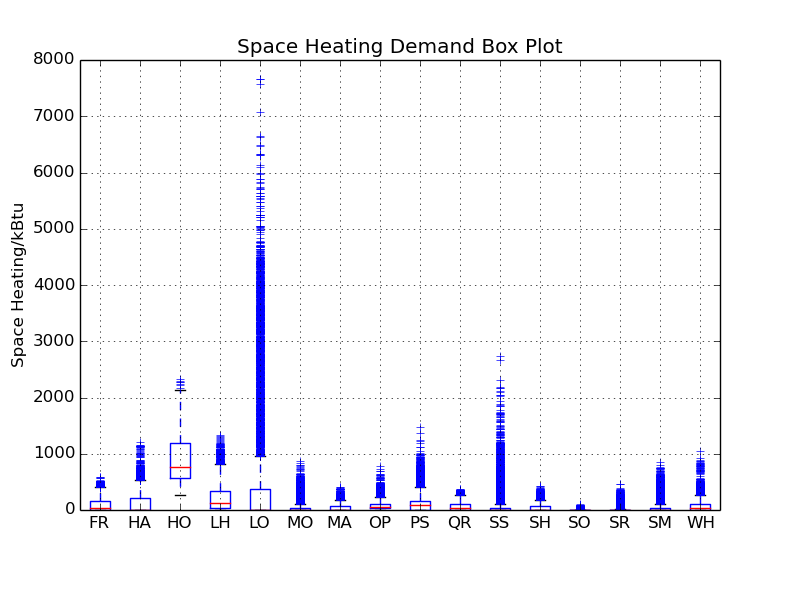
\includegraphics[width=\linewidth]{SH}
  \caption[Space Heating Demand Box Plot]{Space Heating Demand Box
    Plot}
  \label{fig:SH}
\end{subfigure}
~
\begin{subfigure}{0.4\textwidth}
  \centering
  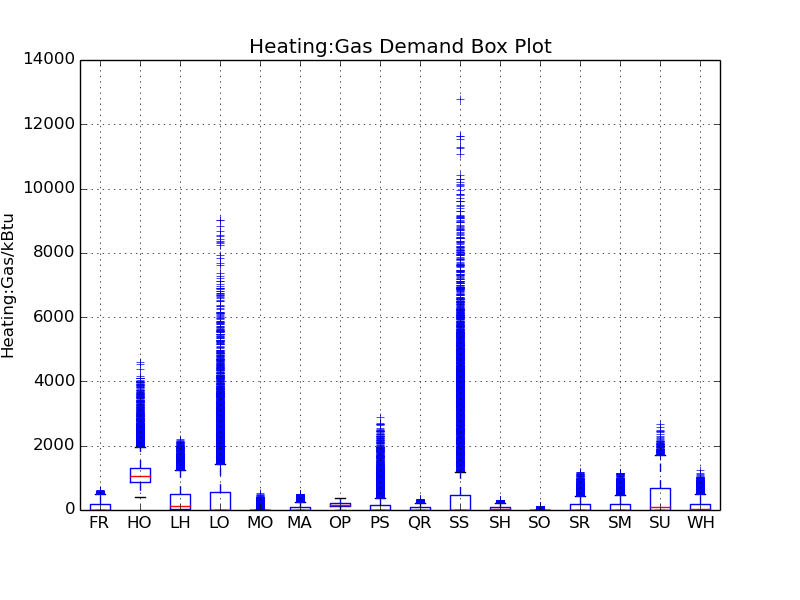
\includegraphics[width=\linewidth]{HG}
  \caption[Heating:Gas Box Plot]{Heating:Gas Box Plot}
  \label{fig:HG2}
\end{subfigure}
\caption[Comparing Heating:Gas and Space Heating]{Comparing
  Heating:Gas and Space Heating}
\end{figure}

Comparing the space heating (Heating:Gas and Heating:Electricity) with
space cooling (Cooling:Electricity), we can see that the heating peak
demand is larger than cooling peak demand for all building types. The
Hospital, Large Hotel and Outpatient Health Care have both the highest
median space heating and cooling demand, indicating a potential for
single building level energy recovery.
\begin{figure}[h!]
  \centering
  \begin{subfigure}{0.4\textwidth}
  \centering
  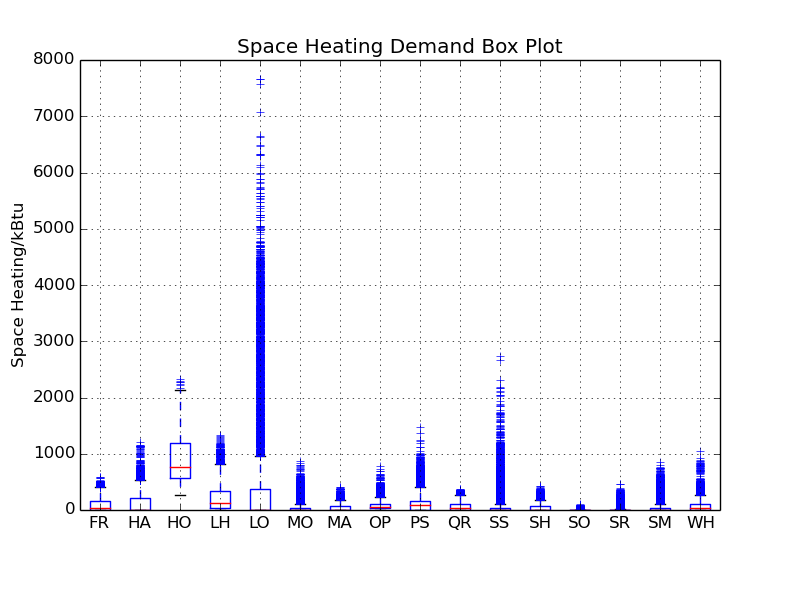
\includegraphics[width=\linewidth]{SH}
  \caption[Space Heating Demand Box Plot]{Space Heating Demand Box
    Plot}
  \label{fig:SH}
\end{subfigure}
~
\begin{subfigure}{0.4\textwidth}
  \centering
  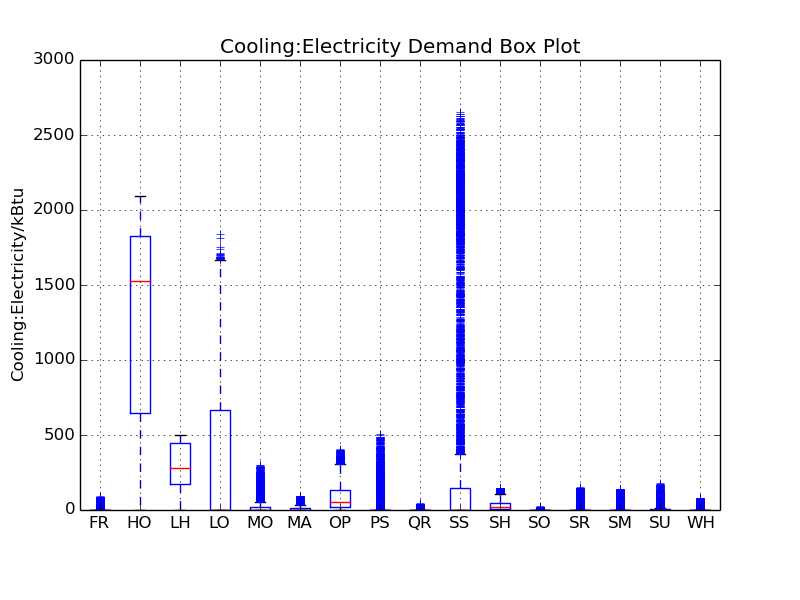
\includegraphics[width=\linewidth]{CE}
  \caption[Cooling:Electricity Box Plot]{Cooling:Electricity Box Plot}
  \label{fig:CE2}
\end{subfigure}
\caption[Comparing Space Heating and Space Cooling Demand]{Comparing
  Space Heating and Space Cooling Demand}
\end{figure}

\subsubsection{Heating Demand vs. Electricity Demand}
Comparing the heat and power demand of each benchmark building type
with the ``heat to power ratio''(HTPR), one of the important
parameters of a CHP plant. Depending on the prime mover types, a CHP
plant can produce 0.6 to 10 unit of waste heat for one unit of
electricity generation~\cite{introCHP2010}. From \fref{fig:HTPR}, we
can see the range of HTPR is from 0 to 25 and the median of HTPR are
all below 1. The building types with a high median HTPR include Large
Hotel, Midrise Appartment, Outpatient Health Care and First Service
Restaurant. Increase the number of buildings with high HTPR ratio is
helpful in more fully reuse of the waste heat from power
generation. In addiction, the large range of Heat to Power ratio also
indicates the necessity of heat storage equipment.
\begin{figure}[h!]
  \centering
  \begin{subfigure}{0.4\textwidth}
  \centering
  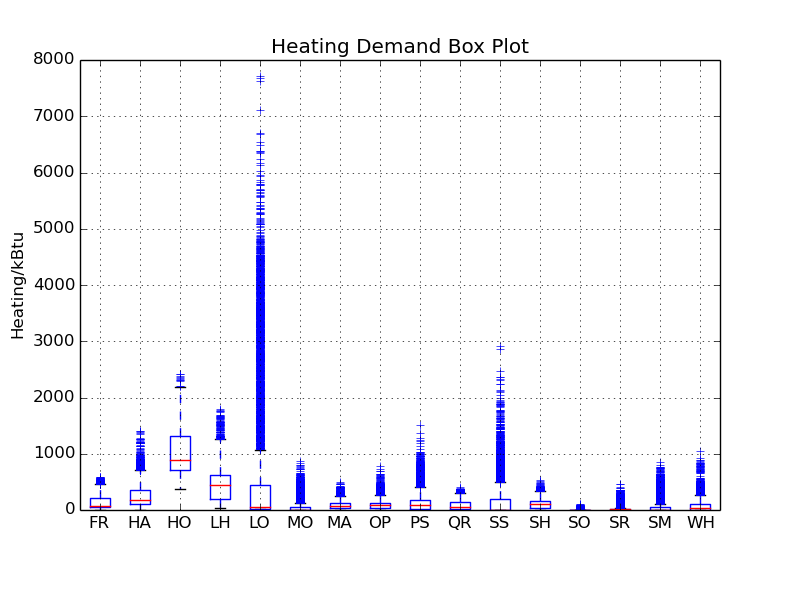
\includegraphics[width=\linewidth]{H}
  \caption[Heating Demand Box Plot]{Heating Demand Box
    Plot}
  \label{fig:H}
\end{subfigure}
~
\begin{subfigure}{0.4\textwidth}
  \centering
  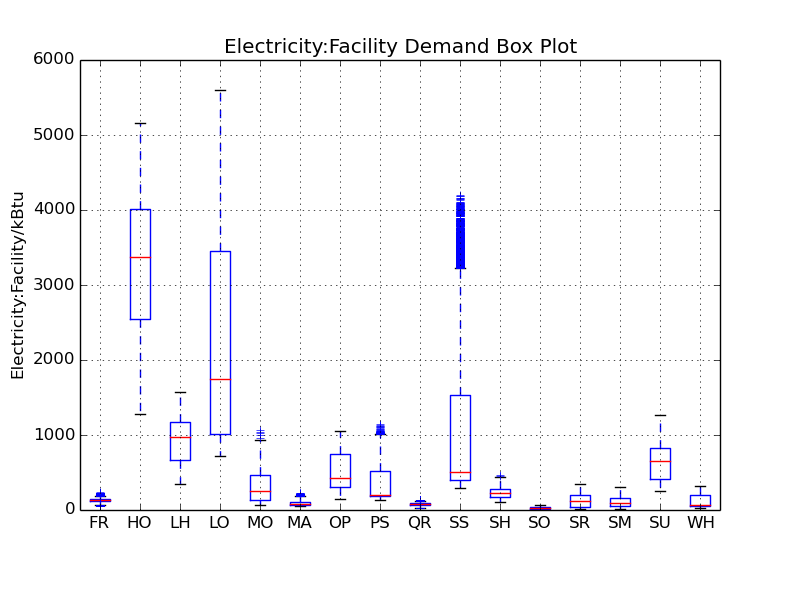
\includegraphics[width=\linewidth]{EF}
  \caption[Electricity Demand Box Plot]{Electricity Demand Box Plot}
  \label{fig:EF2}
\end{subfigure}
\caption[Comparing Heating and Electricity Demand]{Comparing Heating
  and Electricity Demand}
\end{figure}

\begin{figure}[h!]
  \centering
  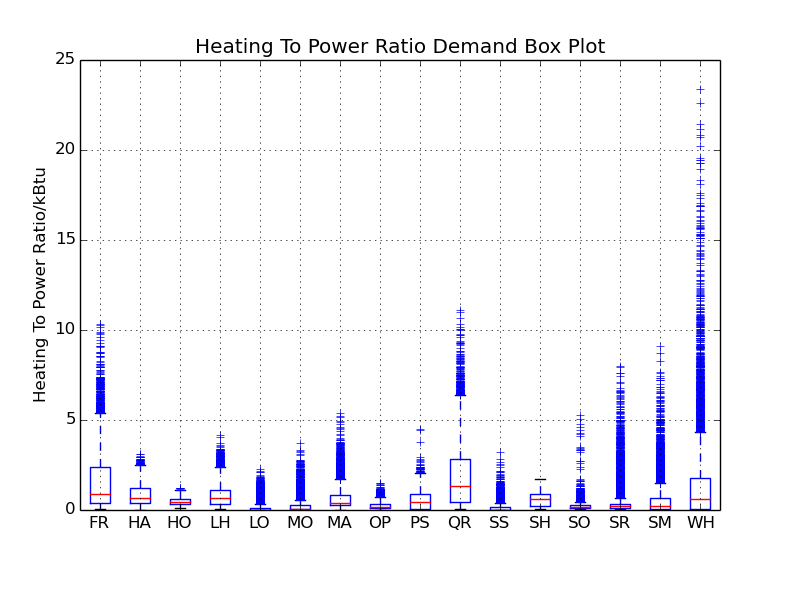
\includegraphics[width=0.7\linewidth]{HTPR}
  \caption[Heat to Power Ratio Box Plot]{Heat to Power Ratio Box Plot}
  \label{fig:HTPR}
\end{figure}%

\pagebreak
\subsection{3D GIS Model Geometry}
The conceptual community model is constructed in
CityEngine~\cite{cityEngine2015}. CityEngine is a software developed
by Esri~\cite{Esri2015}. It can aggregate geographic information into
buildings and is capable of smoothly transition models to
ArcGIS\cite{ArcGIS2015}, one of the widely applied tools for
Geo-referenced data presentation and analysis. Buildings in CityEngine
is defined with ``rules'' using CGA (Computer Generated Architecture)
shape grammar that is unique to CityEngine. The rule-based modeling of
urban environment enables fast construction and easy adjustability of
urban density, skyline and terrain control. It also enables easy
aggregation of Energy profile data into 3D urban environment models,
which is difficult to do in the current ArcGIS, the technical details
will be explained in \aref{AppendixA}.

Although the urban environment in this study is a conceptual setting,
we still want it to reflect the topological and density pattern in a
real urban environment. To construct the model, we first extracted the
topological pattern from an existing urban design project, the Mellon
Arena Project~\cite{baird2014} (\fref{fig:mellonArena}.  There are
eight building types in the project: Residential (43\%), Town House
(2.9\%), Community Center (0.4\%), Commercial (3.8\%), Office (19\%),
Hotel (4.7\%), Cinema (1.4\%) and Garage (24.7\%).

\begin{figure}[h!]
  \centering
  \begin{subfigure}{0.5\textwidth}
  \centering
  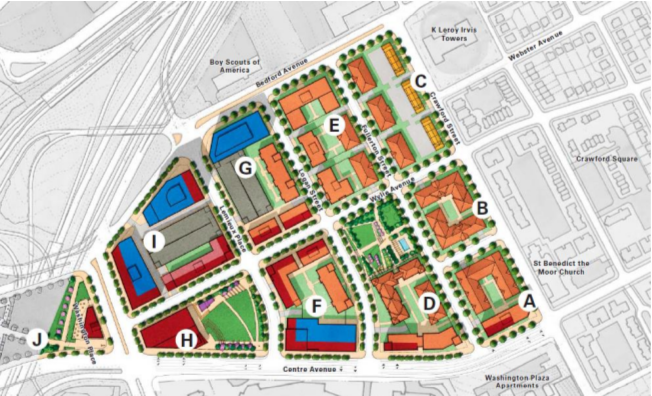
\includegraphics[width=\linewidth]{mellonArena}
  \caption[Mellon Arena Site Plan]{Mellon Arena Project Site Plan View}
  \label{fig:mellonArena}
\end{subfigure}
~
\begin{subfigure}{0.3\textwidth}
  \centering
  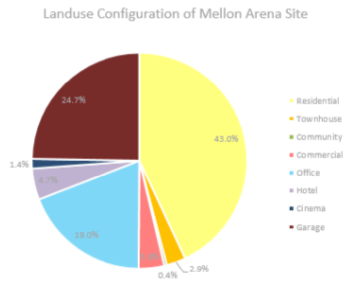
\includegraphics[width=\linewidth]{mellonPie}
  \caption[Mellon Arena Site Land Use]{Mellon Arena Site Land use Configuration}
  \label{fig:mellonPie}
\end{subfigure}
\end{figure}
The 16 building types in DOE commercial benchmark models do not
perfectly correspond to those in the Mellon Arena Site. In order to
adapt the topological pattern of the Mellon Arena Project, a mapping
(function) from building types of Mellon Arena Site to building types
of DOE models is created as is shown in \tref{tab:typeMap}.
\begin{table}[h!]
  \centering
  \begin{tabular}{c| c| c}
    \hline
    Mellon Arena Type &Probability &DOE Building Type\\
    \hline
    \hline
    Hotel &50\%&Large Hotel\\
    \cline{2-3}
    &50\%&Small Hotel\\
    \hline
    Office &30\%&Large Office\\
    \cline{2-3}
    &30\%&Medium Office\\
    \cline{2-3}
    &30\%&Small Office\\
    \hline
    Residential &100\%&Midrise Appartment\\
    \cline{1-2}
    Townhouse &100\%&\\
    \hline
    Commercial &25\%&Full Service Restaurant\\
    \cline{2-3}
    $+$ Cinema $+$&25\%&Quick Service Restaurant\\
    \cline{2-3}
    Community &25\%&Super Market\\
    \cline{2-3}
    Center &25\%&Stand-alone Retail\\
    \hline
  \end{tabular}
  \caption{Mapping of Mellon Arena to Building Types of DOE benchmark model}
  \label{tab:typeMap}
\end{table}

The four major building sectors involved in the current project are
residential, commercial, office and hotel. Their topological pattern
is represented in Figure \ref{fig:mellonTop}. The conceptual model
construction follows the building type topological pattern and the
urban density as the Lower Hill District Project (\fref{fig:sitePlan})

After the land use is assigned (\fref{fig:sitePlan}), one rule file is
applied to all the building lots and generates building geometries by
extruding the building lot (with an offset to the interior) according
to the number of floors of the benchmark buildings. We intend to make
the building geometry simple in order to highlight the color of each
building that encodes its energy demand.

\begin{figure}[h!]
  \centering
  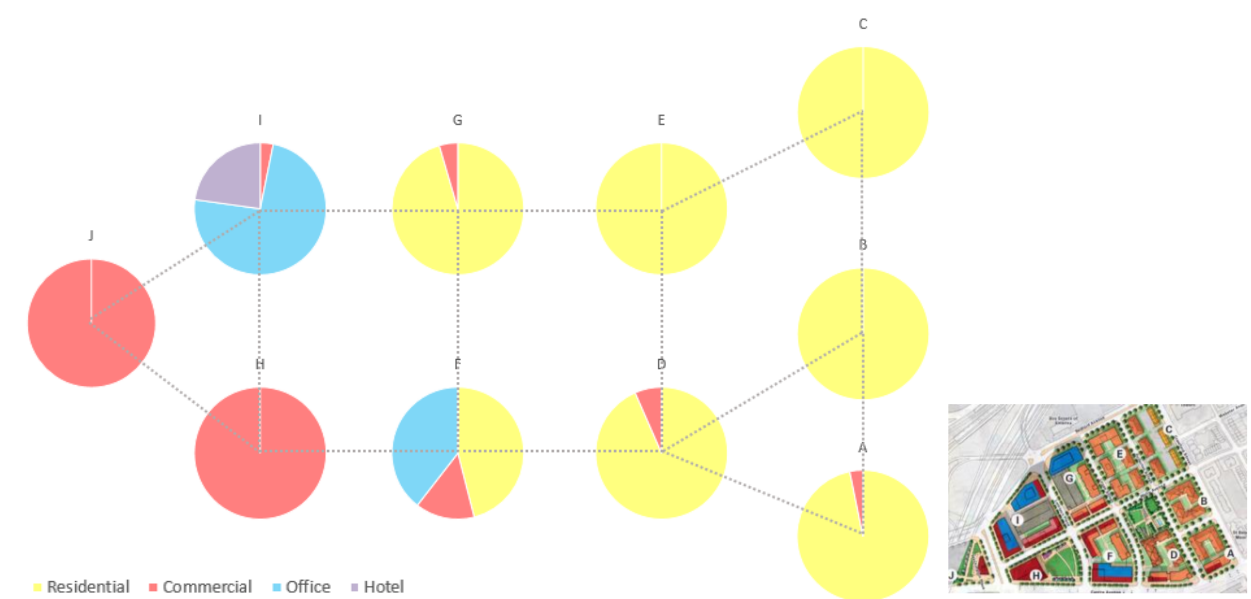
\includegraphics[width=\linewidth]{mellonTop}
  \caption[Building Type Topology]{Building Type Topological Pattern, Mellon Arena}
  \label{fig:mellonTop}
\end{figure}

\begin{figure}[h!]
  \centering
  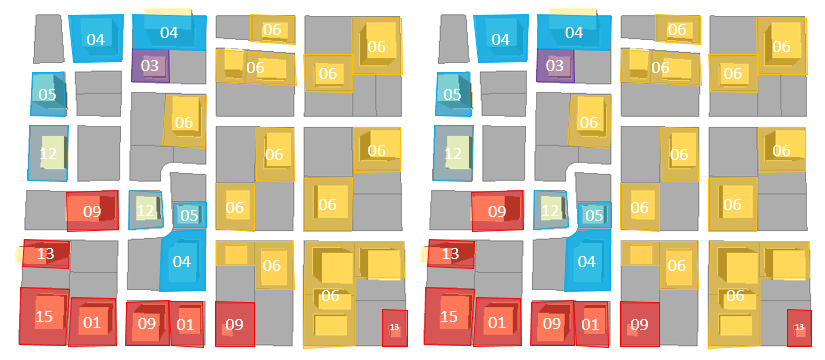
\includegraphics[width=\linewidth]{sitePlan}
  \caption[Conceptual Model Site Plan]{Site Plan of Conceptual Model}~ (01: Full Service
  Restaurant, 03: Large Hotel, 04: Large Office, 05: Medium Office,
  \\06: Midrise Apartment, 09: Quick Service Restaurant, 12: Small
  Office, \\13: Stand-alone Retail, 15: Super Market)
  \label{fig:sitePlan}
\end{figure}

\subsection{Aggregating Hourly Energy Data to 3D GIS Model}\label{sec:aggregateTime}
The authors have experimented with two approaches to aggregate energy
profile data into the conceptual model constructed in CityEngine
\begin{enumerate}[1)]
\item Importing 3D models from CityEngine to ArcScene and aggregate
  the energy data (in the form of a table) into the 3D feature with
  ``one-to-many'' join. For more details please refer to
  \aref{AppendixC}

\item Write the energy profile data directly in the rule file for
  building generation in CityEngine. For more details please refer to
  \aref{AppendixA}

\item Process the color encoding outside of CityEngine and write the
  generated color encoding representations in CityEngine

  This method allows for more specialized symbol and color map
  design. More specific information will be included in the interface
  section X (interface design!!!).

\end{enumerate}

The second approach has the advantage of 1) ready-to-use data
classification method and map symbol templates that facilitates
choropleth map design 2) the ``time-slider'' function for creating a
time-wise navigation and animated map. \fref{fig:arcgisTime} shows the
interface slider and the dynamic map of heating energy demand for the
conceptual model using ArcGIS. There are several problems of this
approach: 1) its high requirement of computational power makes it
infeasible to model or view on a typical PC. The authors only
succeeded in importing the hourly energy profile data when using point
features to represent building geometry. Even for the relatively
simple 3D models in the current study, a relatively higher performance
machine (Dell Precision T1600 Quad Core Intel Xeon, 3.10GHz RAM - 16GB
was used) was used in importing the data, the authors only suceeded in
importing one month of data, never for one year. This technical issue
makes it impossible to using the current ArcGIS platform to implement
high temporal resolution dynamic maps without either truncating time
range or reducing the complexity for building geometry
representation. 2) The time dimension only exist inside the map
file. This means even one produced a dynamic energy map, one cannot
share it without packing all related files and send to others. This
requires the viewer end to have the same high performance
computer. Although the animated map can be exported, the output
animation contains neither any form of temporal label nor the control
of playback. Without time legend, when and for how long the dynamic
changes happen are not shown. 3) For 3D GIS model, it does not contain
a proper function to extract single frames of map images, making it
impossible to implement exterior interface that deals with 3D maps
images.

The first approach, on the contrary, provides more flexibility but
also requires much user-end work including: pre-processing of energy
profile data, implementing data classification method and the
bivariate color ramp. An interface is also needed for visualising the
image sequence.

\begin{figure}[h!]
  \centering
  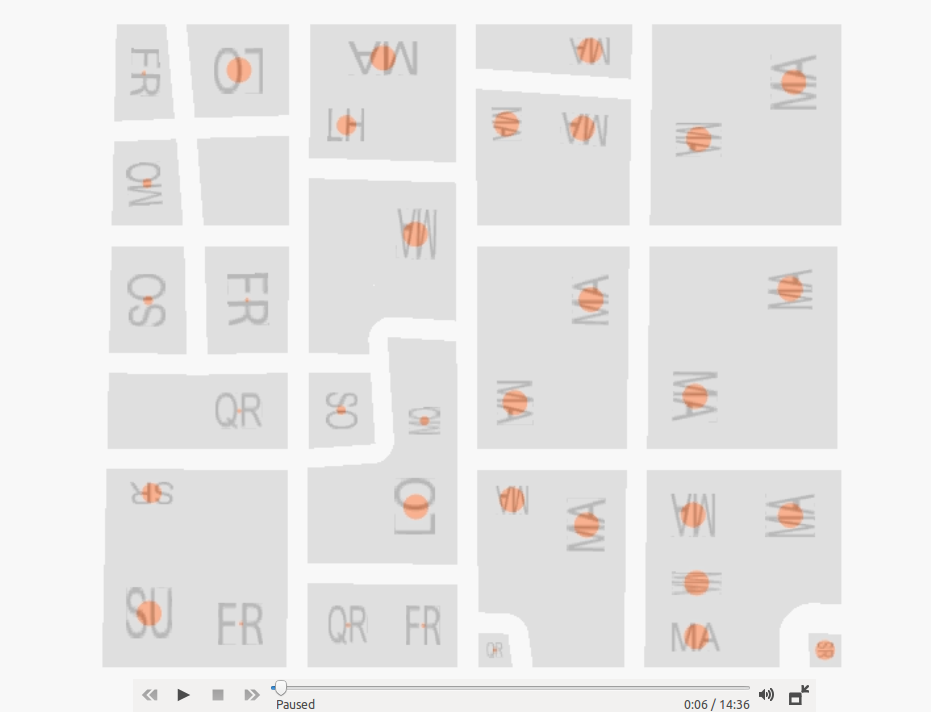
\includegraphics[width=0.5\linewidth]{arcgisTime}
  \caption{ArcGIS Time Slider for Temperal Data Display}
  \label{fig:arcgisTime}
\end{figure}

Due to limited time, the experimented GIS software are only restricted
to ArcGIS and CityEngine. There could be better alternatives to
achieve a dynamic map with more elegance. Find a better alternative
software to implement a dynamic map could be part of the work of the
next stage of the project.

\section{Output Map Images}
Select all the building lot and change their names to ``LOT'' so that
we’ll be able to use the python script to select them all with the
filter ``\texttt{ce.withName(“’LOT’”)}''. Then the map images are
extracted as snapshots from CityEngine with Python script by
iteratively setting the time step and extract snapshot of that time
step:

\makeatletter
\def\verbatim@font{\linespread{1}\tiny\ttfamily} \makeatother
\begin{verbatim}
'''
Created on Jun 5, 2015
@author: yujie
'''
from scripting import *
import time

# get a CityEngine instance
ce = CE()

def main():
    x = ce.getObjectsFrom(ce.scene, ce.withName("'LOT'"))  # < 1s
    for i in range(2):
        for item in x:
            ce.setAttribute(item, 'time', i) # 28 s
            views = ce.getObjectsFrom(ce.get3DViews())  # < 1s
        if i < 10:
            views[0].snapshot(ce.toFSPath('images')+("/img000"+str(i)+".png"))
        elif i < 100:
            views[0].snapshot(ce.toFSPath('images')+("/img00"+str(i)+".png"))
        elif i < 1000:
            views[0].snapshot(ce.toFSPath('images')+("/img0"+str(i)+".png"))
        else:
            views[0].snapshot(ce.toFSPath('images')+("/img"+str(i)+".png"))

if __name__ == '__main__':
    main()
\end{verbatim}
After this step, a sequence of 8760 3D (if using perspective view) or
2D (if using top view) energy images will be extracted and named
according to their time stamp (``imgxxxx.png'' represents the energy
demand for the xxxx-th hour)

\section{Interface Specification}\label{interfaceSpec}
\subsection{User Definition}
First we want to specify a user profile in order to best convey the
information with the Dynamic Energy Map.

The potential category of user group for the Dynamic Map includes: 1)
policy makers, 2) urban planners with the interest in executing
community level energy strategys 3) researchers in energy related
fields 4) public groups or individuals that are involved or interested
in the decision making process of community energy planning.

The target user for the current interface design is restricted to
researchers in energy related fields. The assumption on this user
group about their skill level and background knowledge is that 1) they
have the basic ability to read and understand the layout of a map
environment and can associate it with the urban environment setting
they are associated with 2) they have the ability to correctly
understand moderately complicated map legend and data plot 3) they
have the basic understanding of related concept of building energy
performance attribute and the general implications of these
attributes. The assumptions about their intention is that they might
have different research interest and focus. These assumptions implies
the interface design should: 1) provide both qualitative and
quantitative information; 2) allow for some degree of user control
over data classification, legend selection and full control over time
navigation

\subsection{Goal Function}
The goal function of the interface is in general defined as:
``\textbf{Revealing the spatial-temporal heating, cooling and
  electricity demand variation of the conceptual model with Dynamic
  Energy Map}.''

More specific key goal functions of the dynamic energy map in the
current study is defined as:
\begin{enumerate}[1)]
\item Assisting users to visualize the time dependent hourly thermal
  and electricity demand of each building, each builing sectors and
  the whole community so that they can have a better understanding of
  the importance and the potential of arranging land use pattern and
  building density on the aggregated thermal energy and electricity
  demand of single buildings, building sectors and the whole community.
\item Assisting users to identify the energy recovery opportunities
  through multi-dimensional visualization of the space heating and
  cooling demand.
\item Assisting the sizing of a district energy system CHP plant.
\end{enumerate}

\subsubsection{Function 1: Assisting Energy Recovery}
To achieve this, the space heating and cooling demand should be
represented on the same map that better reveals their correlation.

For the interface design in the current study, the authors used a
bivariate color ramp in energy data representation that depicts the
space heating and space cooling on the same map
(\fref{fig:legend2d}). Red represents high heating demand and blue
represents high cooling demand. The closer the color cell is to the
top, the less heating demand it has. The closer the color cell is to
the left, the less cooling demand it has. The cells on the diagonal
line (purple colored cells) represent the building has relatively
similar heating and cooling demand. The cells to the upper right of
the diagonal means it is heating dominated and the cells to the lower
left of the diagonal means it is cooling dominated. The current
breakpoints are decided through the ``Quantile
method''~\cite{GIS_Jenks2014} for demonstration.

\begin{figure}[h!]
  \centering
  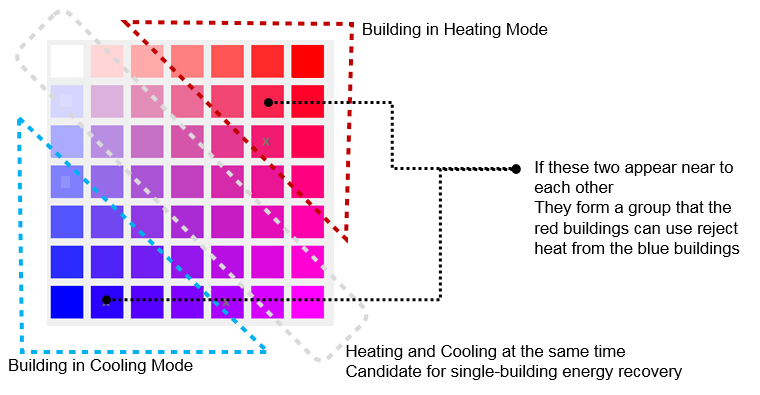
\includegraphics[width=0.5\linewidth]{legend2d}
  \caption[Bi-Variate Color Ramp]{The bivariate color ramp displays
    two variables at the same time: space heating and space
    cooling. It better displays the co-relation between two variables}
  \label{fig:legend2d}
\end{figure}

With the dynamic energy map, the user can first identify those purple
colored buildings directly from the 2D or 3D map as candidate for
building level energy recovering by redirecting the reject heat from
its cooling device condensing coils or cooling towers to the space
that needs heating.

\begin{figure}[h!]
  \centering
  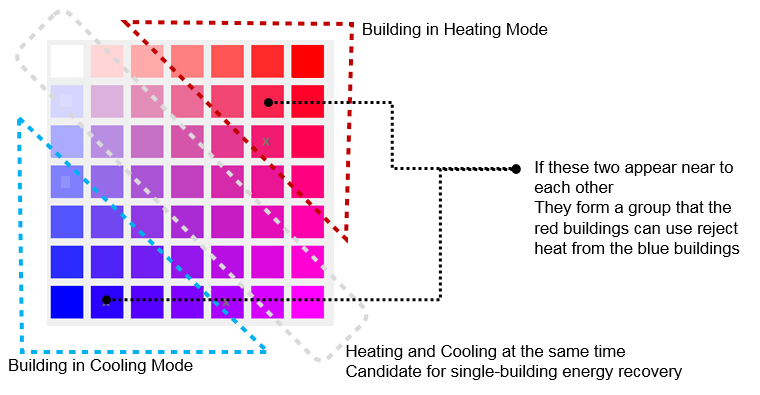
\includegraphics[width=0.5\linewidth]{legend2d}
  \caption[Bi-Variate Color Ramp]{The bivariate color ramp displays
    two variables at the same time: space heating and space
    cooling. It better displays the co-relation between two variables}
  \label{fig:legend2d}
\end{figure}

\subsubsection{Function 1: Assisting Sizing of District Energy System}
As is mentioned in section \ref{districtDesign}, with the Dynamic
Energy Map that depict the spatial temporal load variation, one will
idealy be able to 1) idendify anchor load building, 2) conduct better
design of local load balancing, 3) identify energy recovery
opportunities of the following forms: an individual building with
mixed heating or adjacent buildings with opposite heating and cooling
demand.

\begin{enumerate}[1).]
\item Identify anchor load building
  
  To achieve this function, the map should be able to make the
  building with persistant high heating or cooling demand stand
  out. Thus the design of color scheme that assigns vibrant colors to
  high demand and white to low demand. The break points of ``high''
  demand remains to be decided in further project development. For the
  current implementation, the break point is acquired with quantile
  classification method with.

\item Local load balancing
  
  To achieve this, the first step would be to enable users to select a
  subset of the existing buildings and the program will calculate the
  aggregated load and plot the curve for the aggregated load of the
  selected building group (within the specified time period).


\end{enumerate}

\subsection{Specification of the Major Operation}
The desired major operations for the target user include: 
\begin{itemize}
\item Map display and data plot
\item Navigation utilities that navigates through dynamic map and data
  plot
\item Provide default settings for choropleth map display
\end{itemize}

\subsubsection{Map display and data plot}
For researchers or planners: The desired map display should be a 2D
and 3D map (providing easy toggle between 2D and 3D map or align the
two representations side by side) with graduated symbol or color
representing the heating or cooling demand. The map display should
also be coupled with corresponding data plot or data statistics that
providing the quantitative insight that supports design decisions.

For general public: The desired map display should be a 3D map
. Instead of using data plot, a more intuitive bar chart of the
aggregated demand could be more helpful in presenting a general
idea. The bivariate choropleth map legend should also be replaced with
two color ramps or even with only colors of extreme value. The data
classification method should also be chosen so that the peak
occurrence time is emphasized rather than the absolute energy
consumption value.

\subsubsection{Navigation utilities that navigates through dynamic map
  and data plot}
The ability to navigate through a series of map images and present
dynamic data plot accordingly, is the basic function that differs
the current work from a static map. Some desired behavior of the
slider includes:
\begin{itemize}
\item Linear and cyclic time representation. According to section
  \ref{anime}, the time has both linear and cyclic aspect. The time
  navigation utility should provide both ``linear'' time navigation
  and ``cyclic'' time navigation. This requires a global time
  navigation that accounts for the linear aspect: it can go through
  the whole time period with the highest time resolution. It also
  requires a series of default time steps settings corresponding to
  the natural recurring pattern of the energy usage profile
\item Another desired feature is providing adjustable auto-play of the
  map animation. The reasoning behind this is the debatable level of
  user control in the study of Johnson and Nelson~\cite{Nelson1998},
  when they argue that allowing arbitrary time control might degrade
  the ability of animated map on conveying temporal pattern. This
  feature is to be implemented in future development of the project.
\end{itemize}

\subsection{Provide default settings for choropleth map display}
Creating several default settings for choropleth map display,
i.e. provide choices for data classification and color mapping. For
the current implementation, the variables in display is the heating
and cooling energy consumption profile. The customization choices only
restrict to the two classification method: even or quantile
method. The color ramp is predefined to be a bivariate color ramp from
white to red and blue. For later stages, a desired behavior would be
to provide the full control of color settings.

\subsection{Guidelines from Literature Study}
Here we summarizes some of the design choices made according to
related literature research on dynamic map design:
\begin{itemize}
\item Provide both 2D and 3D map display as a result of the debating
  situation mentioned in section \ref{2d3d}.
\item Choose bivariate choropleth map representation which has the
  highest accuracy rate in map reading experiments~\cite{Elmer2012}.
\item Providing the most commonly used data classification method:
  Equal Interval and Quantile Interval~\ref{dataClassification}
\item The number of classes for energy data classification is chosen
  to be 7, less than the suggested value of 10 as a result of smaller
  display size than 1024x768~\cite{doi:10.1559/1523040639298}
\item Provide both linear and periodical navigation based on section
  \ref{timeRepresent}
\item Using the principle of ``dual coding''~\cite{Resch2014} to
  assist legend reading by section \ref{anime}.
\item Noise removal in map display of energy profile
  data~\cite{Dorling1992}. This is done through the discrete color
  scheme design.
\end{itemize}
